%%% paper.tex — PLOS 2026 submission
%%% ACM sigplan, anonymous, 10pt (per CFP)
%%% Max 6 pages (excl. bibliography), double-blind
\documentclass[sigplan,screen,10pt]{acmart}

% Disable CCS, keywords, and ACM ref format (not required for submission)
\settopmatter{printacmref=true}
% \renewcommand\footnotetextcopyrightpermission[1]{}
% \pagestyle{plain}

% PLOS 2026 venue info (replaces the default acmart "Conference'17" placeholder).

\copyrightyear{2026}
\acmYear{2026}
\setcopyright{cc}
\setcctype{by}
\acmConference[PLOS '26]{14th Workshop on Programming Languages and Operating Systems}{September 29-October 02, 2026}{Prague, Czech Republic}
\acmBooktitle{14th Workshop on Programming Languages and Operating Systems (PLOS '26), September 29-October 02, 2026, Prague, Czech Republic}
\acmDOI{10.1145/3831586.3838143}
\acmISBN{979-8-4007-2877-8/2026/09}

\acmSubmissionID{10}
% Enable the auto-generated ACM Reference Format block.
% \settopmatter{printacmref=true}
\settopmatter{authorsperrow=2}


% CCS Concepts (replicated from the 2025 OSmosis paper)
\begin{CCSXML}
<ccs2012>
<concept>
<concept_id>10010147.10010341.10010342.10010344</concept_id>
<concept_desc>Computing methodologies~Model verification and validation</concept_desc>
<concept_significance>500</concept_significance>
</concept>
<concept>
<concept_id>10011007.10011074.10011099.10011692</concept_id>
<concept_desc>Software and its engineering~Formal software verification</concept_desc>
<concept_significance>500</concept_significance>
</concept>
</ccs2012>
\end{CCSXML}

\ccsdesc[500]{Computing methodologies~Model verification and validation}
\ccsdesc[500]{Software and its engineering~Formal software verification}



% Keywords
\keywords{Hardware Model Validation, Software Verification, Complexity Reduction.}% 

%%%%%%%%%%%%%%%%%%%%%%%%%%%%%%%%%%%%%%%%%%%%%%%%%%%%%%%%%%%%%%%%%%%%%%%%%%%%%%%
% The Venue this Paper will Appear in
%%%%%%%%%%%%%%%%%%%%%%%%%%%%%%%%%%%%%%%%%%%%%%%%%%%%%%%%%%%%%%%%%%%%%%%%%%%%%%%




\usepackage{cleveref}
\usepackage{enumitem}
\usepackage{lipsum}
\usepackage{float}
\usepackage{listings}
\usepackage{soul}
\usepackage[most]{tcolorbox}

\newfloat{lstfloat}{htbp}{lop}
\floatname{lstfloat}{Listing}
\def\lstfloatautorefname{Listing} % needed for hyperref/autoref

\setlength{\abovecaptionskip}{4pt}
\setlength{\floatsep}{10pt}

%
% \setlength{\abovedisplayskip}{0pt}
% \setlength{\belowdisplayskip}{0pt}
% \setlength{\abovedisplayshortskip}{0pt}
% \setlength{\belowdisplayshortskip}{0pt}

\begin{document}

%\title{The Crux about Hardware Model Validations -- Towards Efficient Model Validation on Real Hardware}
\title{Towards Tractable Hardware Model Validation Against Real Hardware}

\author{Rishika Varma Kalidindi}
\orcid{0009-0009-5971-8715}
\authornote{Work done while at the University of Michigan and MPI-SWS.}
\affiliation{%
  \institution{University of Texas at Austin}
  \city{Austin, TX}
  \country{USA}
}

\author{Reto Achermann}
\orcid{0000-0003-3263-7236}
\affiliation{%
\institution{Technical University of Munich}
% \department{Department of Computer Science}
\city{Munich}
\country{Germany}
}

\begin{abstract}
%%
%% Abstract %%
%

% Context
Verifying low-level systems code requires reasoning about how software interacts with the hardware environment it runs on.
Typically, this means specifying an abstract model of the hardware and verifying the code against it. 
However, the validity of the verification result depends on the accuracy of the formalized hardware model.  
%
% Problem
Unfortunately, validating the accuracy of the formalized hardware model is hard. It not only requires relating the model's specification to the observable behavior of real hardware, but also involves many invisible internal microarchitectural steps that influence the observable execution of a modern processor. 

% Approach
We present a methodology that lets us validate an abstract formal model against real hardware by generating test cases, executing them on real hardware to capture traces of observable behavior, and finally employing a synthesis approach to identify the internal microarchitectural steps that explain the observable behavior. 
To scale this approach to real-world examples, we employ a state-reduction method to limit the possible choices for test case generation and synthesis.
% Results
We evaluate this methodology on a model of the x86 MMU, demonstrating that synthesis can recover internal microarchitectural steps that explain observed hardware behavior.
\end{abstract}

\maketitle

% Page Budgets: 6 pages total
%%%%%%%%%%%%%%%%%%%%%%%%%%%%%%%%%%%%%%%%%%%%%%%%%%%%%%%%%%%%%%%
\section{Introduction}\label{sec:intro}    % About one page
%%%%%%%%%%%%%%%%%%%%%%%%%%%%%%%%%%%%%%%%%%%%%%%%%%%%%%%%%%%%%%%

%
% Context:
%  - Verification of system softare
%  - hardware model to verify against
% 
System software is a high-value target for formal verification due to its critical role in enforcing isolation between processes, containers, or virtual machines.
There has been a steady stream of verified kernels
~\cite{Klein:2009:seL4, Gu:2016:CertiKOS, Chen:2025:Atmosphere}, hypervisors~\cite{Tao:2021:seKVMArm}, or security monitors~\cite{Zhou:2024:Verismo}.
Common to all system software is that it must directly interact with hardware to establish the desired isolation properties, e.g., set up a virtual machine or the address space of a process. 

Verifying system software means reasoning about the effects of its interactions with hardware.
This means that we must write an abstract specification of \emph{relevant} parts of the hardware platform and its behavioral semantics, e.g., control registers, the translation lookaside buffer (TLB), the mechanics of a page table walk, or the semantics of the virtual machine control structure fields. 
Then use this specification to reason about the effects of a write to a register or a page table entry on the overall system, e.g., whether the process now has access to a given page of memory.
Consequently, the verification result depends directly on the accuracy of the hardware specification it is verified against.


%
% Problem:
%  - documentation is incomplete, contradicting
%  - environment can contain bugs
%  - do not express relevant aspects
%  - 
Unfortunately, writing accurate hardware specifications is hard on its own, as documentation is often incomplete, imprecise, or even contradictory. 
There are three main problems: 
First, the formal specifications of the environment contain bugs~\cite{Fonseca:2017:EnvironmentBugs} that manifest in the verified implementation~\cite{goldweber2024ironspec,reid2016trustworthy}.
Second, there is a reality gap between the formal model and the actual hardware~\cite{Gleirscher:2019:RealityGap}, i.e., the formal model does not contain bugs, but it is either too permissive or too restrictive. The verification effort becomes much harder than necessary, or overapproximates relevant details.
Third, not all the steps the hardware takes are directly visible to the software. However, they influence observable outcomes. For example, a speculative TLB fill walks the page table and inserts an entry in the TLB that might be used in a future memory access. 

It is paramount that we do not take hardware specification solely on faith, but 
validate the formal specification against real hardware implementations~\cite{reid2016trustworthy,armstrong2019sail}. 
The benefit is two-fold: a mismatch can mean a bug in the specification or the hardware itself. 
Existing validation approaches cover the ARMv8 architecture specification~\cite{Reid:2017:ValidationArmv8},
TSO memory model~\cite{owens2009x86tso} or the Arm weak memory models~\cite{alglave2011litmus,alglave2014herding}.
However, none of them explicitly included the invisible, processor internal steps of the virtual memory system.

%
% Approach:
% - methodology to validate the hardware model
% - state reduction techniques
% - 
%
We describe a methodology for validating hardware models against real hardware. 
On a high-level, this includes 
1) test case generation based on an operational model,
2) execute these test cases on real hardware, and
3) validation of the model against a trace of observed hardware behavior.
During validation, we need to find the \emph{missing} invisible hardware steps needed to justify the observable trace. 
We cast this into a software synthesis problem. 
However, instead of synthesizing instructions, we synthesize the invisible, internal hardware steps and use the observable trace as the verification condition.

Exhaustively exploring all possible hardware behaviors is prohibitively expensive.
Hence, we must reduce the number of choices for test case generation and synthesis-based validation.
To reduce the number of choices in test case generation and validation, we employ techniques that leverage symmetry and abstraction.
Intuitively, we can replace a trace with a simpler one if it still exposes the same hardware behavior.
For example, consider an execution trace of memory accesses in an eight-core system; we might be able to find an equivalent trace on a four-core system by combining the execution steps accordingly.
e
% 
% Results:
%
We validate our approach using a model of the x86 memory management unit that models the translation lookaside buffer, page walk caches, page-table walks, speculative TLB fills, and TSO-memory semantics. 
We cover test-case generation, trace collection, and trace validation against this model. 
Finally, we present our choice-reduction techniques that reduce the number of cores, virtual pages, physical pages, and page-table entries. 

% 
% Contributions
%
The contributions of this paper are:
\begin{itemize}
 \item An overall methodology to systematically validate a model against real hardware. 
 \item A trace-based validation technique using a synthesis approach.
 \item An approach to reduce the number of choices in test-case generation and validation.

\end{itemize}

 

% To be able to verify the correctness of an application’s code has 
% many aspects. While the application’s own code is an integral aspect, 
% it is almost equally important for the application code to ensure that 
% the process environment is used correctly. This implies that we need 
% user process leverageable models of the process environment including 
% the operating system part and the hardware part. While the operating 
% system model part of the process environment can be derived from a 
% reduction of a verified specification of the operating system code, the 
% hardware model is not as straightforward. Documentation can help in 
% proposing a hardware model however, these are often lacking and 
% existing practices may be incorrect. Prior work on trustworthy processor
% specifications argues that formal environments must be validated against
% implementations, not taken on faith~\cite{reid2016trustworthy,armstrong2019sail}.
% Thus, to ensure correct process environment specifications for applications to leverage, it is 
% essential that it is based upon a tested and robust hardware model. To 
% this end, we propose an initial exploration of the different aspects 
% required to validate a hardware model. We discuss how we use these 
% methods and our observations for the x86 paging hardware.

% Testing the hardware model comes with challenges that are unique to 
% this scenario: In verifying software traditionally, we are able to 
% observe and identify every action that leads to a transition in state 
% defined by our model. In the case of the hardware model however, there 
% are many events that are triggered and happen within the hardware that 
% are not directly observable. Thus, we need to test that our model 
% encompasses observed behaviours using externally visible actions and 
% anticipating the internal events that can explain the behaviour seen. 
% For eg: in the case of paging, a partial page walk being cached is not 
% observable, however if this cached page walk is used later to complete 
% the page walk and read data memory, then depending on if the current 
% page writes do not match the observed read, the caching can be inferred.


% \subsection{Approach}\label{sec:intro:approach}
% We discuss the approaches that we explored in addressing each of these aspects. The test cases for this model are in the form of traces of externally invocable actions that correspond to the externally visible actions in the model, eg: writing a page table entry, reading data memory, etc. Instead of the traditional approach of handcrafting various litmus tests that target interesting scenarios~\cite{owens2009x86tso,alglave2011litmus,alglave2014herding}, we sought to automate the generation of a sufficiently exhaustive set of traces which encompass all possible behaviours.
% % TODO: test cases part
% To execute the test traces to obtain corresponding results, we built a test harness using the barrelfish operating system ensuring that we execute as close to the hardware as possible. 
% Finally, we propose the idea of approaching verification of a trace against the model as a synthesis problem. The model itself dictates the constraints which are derived from the states and transitions, and the externally observed events (along with the outputs from the test execution) guides generation of potential internal state transitions that justify the observed behaviour. In the case that we do not find any such completed traces, it indicates a violation in the model and can direct improvement of the model. 

% We show some preliminary evaluations of the promise our approach holds in reducing the test space and the trace analysis of the model validation by showing simple examples of improving confidence of our correctness in these aspects which can be extended to larger traces and more complex models.


  % 1.0 pages (including abstract)
%% ============================================================
\section{Background: x86 Processor Architecture}\label{sec:background}
%% ============================================================

%
% Here, we may need to give a high-level primer on the x86 memory 
% subsystem, store buffers, memory ordering, fences, and internal events.
%

% how memory address translation works
\noindent\textbf{Memory Address Translation}
The x86 MMU translates virtual addresses used by programs into physical addresses understood by the hardware at the granularity of pages: continuous, naturally aligned regions of memory 4KiB, 2MiB, or 1GiB in size.
The page table, a memory-resident, multi-level radix tree, stores this address mapping.

% translations can be cached
\noindent\textbf{Translation Caching.}
The x86 MMU has two kinds of per-core caches that speed up address translation: 
1) the translation lookaside buffer (TLB) stores the result of successful page table walks, and 
2) page-walk cache (PWC) stores partial page table walks. 
TLB hits bypass the page walk entirely, while a hit in the PWC skips some levels of the page table.
Moreover, the page table walk itself uses the processor's data caches.
The TLB and PWC are non-coherent. The OS must explicitly invalidate stale entries after a page table update.


% the memory model that makes things slightly more complicated
\noindent\textbf{Store Buffer and Memory Model.}
The processor implements a store buffer that records memory writes before they are written to the cache, thereby making them globally visible through the cache coherence protocol. 
The processor can retire store instructions without waiting for the memory subsystem.
However, writes sitting in the store buffer are not visible to other cores, while the store buffer is snooped and returns the last-written value for subsequent same-core reads.
%
The x86 architecture follows a \emph{Total Store Order (TSO)} memory model~\cite{owens2009x86tso, sewell2010x86tso}, meaning that the hardware guarantees that memory writes become visible in the same order as they are emitted to the store buffer.
%
Serializing instructions (e.g., fences) force store buffer writeback.


% talk about processor internal events
\noindent\textbf{Processor Internal Events.}
A processor effectively executes a sequence of events that we can classify as externally observable or invisible internal microarchitectural events.
Instruction execution is an observable event with a well-defined outcome, e.g., a memory read returns the value 42, which gets copied into a register.
Internal events such as cache fill/eviction, store buffer writebacks, and speculative execution are not directly observable, but they might influence the outcome of an observable event. For example, the processor speculatively executes a TLB fill, resulting in a TLB hit on the next memory access.     % 0.5 pages
%% ============================================================
\section{Why Accurate Hardware Models Matter}\label{sec:motivation}
%% ============================================================

Verifying operating systems is particularly challenging because they directly interact with hardware to configure security-relevant features, such as virtual memory.
These interactions can change which memory regions are accessible and which are not. 
To reason about isolation properties and system integrity, one must formally specify the semantics of the underlying hardware environment and analyze the operating system's interaction with it. 

\subsection{A Simple Model, and its Problems.}

Recall, to unmap a memory page, the operating system must invalidate the corresponding page table entry by setting its present bit to 0. However, this alone is not sufficient, as the TLB might still cache the now-stale translation. 
We could model the system as two flat mathematical maps: one representing the TLB and one storing a flattened representation of the page table's virtual-to-physical address translation. Then define operations to update a page table entry, fill and invalidate the TLB, and perform a memory access that uses the translation information in the TLB. 
%
Unfortunately, this model has several problems in accurately depicting certain important behaviors.

\noindent\textbf{Problem 1: Over-Aproximation.} 
The page table is a flat mathematical map. Updates to intermediate levels in the page table structure are abstracted away. TLB fills are atomic. 

\noindent\textbf{Problem 2: No Memory Model.}
Store buffers and data caches are omitted. Updates to the page table are atomic and become globally visible to all cores simultaneously.

% and the TLB could be filled using the old page table entry.
% Updates to the page table are memory writes that are governed by the underlying memory model.

\noindent\textbf{Problem 3: Missing Internal Microarchitectural Steps.}
The hardware may speculatively evict and/or fill the TLB, or write back a store buffer entry, at any time, even while updates to the page table are in progress. As a result, the MMU may not see updates to the page table immediately. Thus, it may map a virtual address to the wrong physical address or apply the stale (wrong) permissions during access control, breaking isolation and violating system security.

\subsection{The Core Problem: Model-Reality Mismatch}

There are two kinds of mismatches:

\noindent\textbf{1) Hardware steps outside of the modeled behavior.}
The formal model abstracts away relevant underlying details (e.g., page table structure, store buffers, non-atomic updates) or overly constrains its operations (e.g., by preventing certain memory reorderings that are possible on weak-memory hardware).
Consequently, hardware may exhibit behavior for which there exists no corresponding step in the specification, and verification against such an overapproximated specification yields an implementation that does not correctly handle behavior present on real hardware. This results in undefined behaviors, potentially causing security violations.

\noindent\textbf{2) Model Specification is too Broad.}
The formal model is more permissive than the real hardware. For example, it allows arbitrary reorderings of memory writes while the hardware enforces a total-store order. 
While this covers all behavior of the underlying hardware, it also forces reasoning within a less permissive environment specification, which may make the proof effort more substantial or impractical.


\subsection{The Environment Specification must be Tight}

The environment specification should express the hardware's possible behavior, nothing more.
A too-strict model yields meaningless verification results because the verified program runs in an environment it cannot handle, and its subsequent behavior may diverge from expected, safe patterns~\cite{goldweber2024ironspec, reid2016trustworthy}. 
While an overly permissive environment specification might lead to a more complicated verification effort or even less performant code due to unnecessary synchronization.

% \noindent\textbf{Take-Away:}
% It is paramount that we do not take hardware specifications solely on faith, but 
% validate the formal specification against real hardware implementations~\cite{reid2016trustworthy,armstrong2019sail}. 

    % 0.5 pages
% ------------------------------------------------------------
%                              % 2.0 pages until here
% ------------------------------------------------------------ 
%% ============================================================
\section{Design}\label{sec:design}
%% ============================================================

{\color{red}\textbf{Reto is currently working here.}}

\autoref{fig:validation-pipeline} shows the overview of our model validation pipeline.
The goal is to systematically validate the hardware model against real hardware. 
The validation pipeline consists of a test-case generator, a test execution harness, a trace validator. 
The input to the pipeline is a reduced hardware model that provides the basis for generating the test programs and trace validation.
Next, we elaborate on the purpose of each component in the validation pipeline.

\begin{figure*}[t]
    \centering
    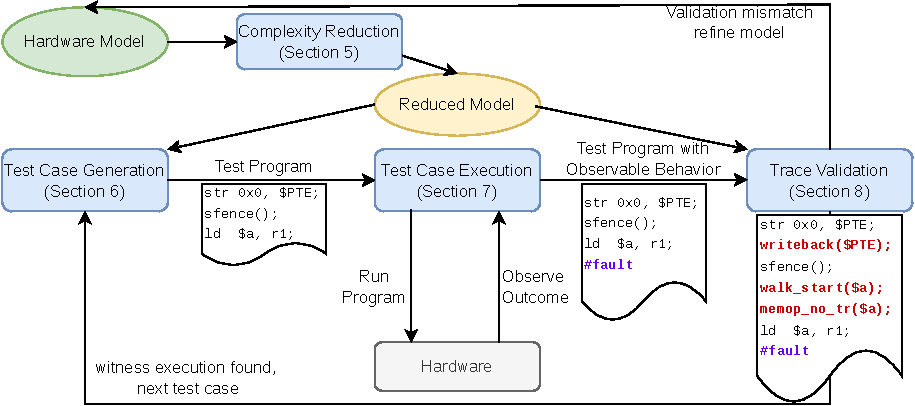
\includegraphics[width=\columnwidth]{figures/SystemOverview.drawio.pdf}
    % TODO refine. 
    \caption{Overview of the validation methodology. The formal model and
    reduction argument constrain both test generation and trace analysis;
    the harness connects stimulus traces to observations on real hardware.
    {\color{red}\textbf{Probably need to make this a bit nicer... maybe include something that hints at the internal steps}}
    }
    \label{fig:validation-pipeline}
\end{figure*}

\noindent\textbf{Hardware Model} 

\noindent\textbf{Model Reduction}

The model is expected to be consistent across variables like the number of cores, virtual addresses, physical addresses, and trace length. However, testing it across every possible value of these variables is impractical, and synthesising hidden steps for long traces causes a state-space explosion that quickly becomes computationally inviable. We therefore propose a number of informal reduction arguments that identify small representative configurations that still seem capable of exposing the behaviours we care about. These are similar in spirit to small-world or small-scope arguments, where behaviours in a large state space are often expected to have small witnesses. The concrete bounds and the per-resource arguments behind them appear in \Cref{sec:reduction}.

\noindent\textbf{Test Case Generation}

The formal model (\Cref{sec:model}) together with our proposed reduction argument (\Cref{sec:reduction}) constrain a test-case generator that emits observable stimulus traces. We chose to automate generation over hand-written litmus tests approaches such as those in~\cite{owens2009x86tso,alglave2011litmus,alglave2014herding}.

 Generate diverse stimulus traces that expose interesting hardware behaviours while staying within bounds. We ensure this by using our reduction arguments to constrain the test case generation process. The generator emits only externally invocable actions such as data memory operations and page table writes, since these are the only events the harness can issue.

\noindent\textbf{Test Execution Harness}

 These stimulus traces are then executed on real hardware via a lightweight harness, producing an observable execution trace including the values returned by data memory operations(reads and writes). 

 Execute each stimulus trace on the hardware under as much isolation as practical, so that the observed read values reflect translation and caching effects in hardware rather than interference from the operating system. 

\noindent\textbf{Trace Validation}

The observable trace is handed to a synthesis-based trace analyser that searches for a sequence of model transitions whose observable projection matches our observed trace. A successful search yields a witness execution (including hidden steps) that explains the observation and counts as a positive validation. A failed search indicates that no model-admissible execution exists for that observation, which is evidence that the model is incorrect or incomplete and can direct improvements. We chose a synthesis encoding of trace checking because the gap between observed and internal traces is exactly the kind of hidden-step reconstruction problem solvers handle well (\Cref{sec:bg:synthesis}).

 Decide whether an observed trace is explainable by the model. We cast this as a synthesis problem such that given the model's transition relation and the observed externals, we try to find a sequence of internal steps that ties them together.
        % 0.3
%% ============================================================
\section{Proposed Model}\label{sec:model}
%% ============================================================

\subsection{Formal Hardware Models}\label{sec:bg:formal}
{\color{blue} moved here for now...}
Our goal is to capture the behaviour of the hardware as a model consisting of states and transitions between them. Concretely, we view a hardware model as a state-transition system. Transitions are labelled by actions, which we divide into \emph{observable} actions (externally invocable or externally visible events) and \emph{internal} actions.

This separation lets us talk about two related traces. An \emph{observable trace} records only externally visible events,
\[
o_1, o_2, \dots, o_n,
\]
while an \emph{internal execution} records the full sequence of model steps,
\[
i_1, i_2, \dots, i_m.
\]
We write \(\pi\) for the projection that erases internal steps and keeps only observable events, so that \(\pi(i_1 \dots i_m) = o_1 \dots o_n\). We say the model \emph{explains} an observed trace if there exists an internal execution in the model whose projection matches that trace. This yields an \emph{explainability} relation between observed behaviour and the model.

% Also add a representation explanation for stimuli traces

This paper focuses on \emph{model validation} rather than using the model as a trusted oracle. Informally, a hardware model is correct if every observable behaviour produced by the processor can be explained by some execution in the model. Equivalently, the model should not rule out any behaviour the hardware can actually exhibit.


The paging hardware is modeled as a state-transition system. The essence of the model is detailed below:

\begin{itemize}
    \item Writes to the page table are buffered in a store buffer and overall execution follows Total Store Ordering (TSO).
    \item Translation is performed via page walks which are non-atomic and in the form of defined walk steps.
    \item Translations are cached in a per-core Translation lookaside buffer (TLB) which is indexed by the virtual address. This may not be coherent with the page table in memory.
    \item Partial page walks may be cached within each core and reused as a prefix in a subsequent walk.
\end{itemize}
         % 

\section{Reduction Argument}\label{sec:reduction} %%

The model is expected to be consistent across variables like number of cores,
virtual addresses, physical addresses, etc. However, testing the model across
every possible value of these variables is impractical. Testing the model on
very large traces with many external and internal actions also causes state
space explosion and quickly becomes computationally inviable. Thus, for the
purpose of generating tests, we explore how far the testing space can be
reduced and we propose a number of informal arguments to reduce the testing space. While these arguments are not complete proofs of sufficiency, they are working reduction arguments which try to identify small representative configurations that still seem capable of exposing the behaviours we care about. Robust proofs would be necessary before these bounds could be treated as complete or final. For the proof-of-concept model, however, these arguments give us a principled way to keep the generated tests tractable. This is similar in spirit to small world or small scope arguments, where behaviours in a large state space are often expected to have small witnesses.

The aspects that we consider relevant to this model that need consideration are:

\begin{itemize}
  \item Number of cores 
  \item Number of paging levels 
  \item Number of virtual addresses 
  \item Number of physical addresses for data
  \item Number of physical addresses for page-table entries 
  \item Length of each trace
\end{itemize}

For each of these aspects, we ask what the smallest non-obviously-unsound
bound seems to be. In other words, we try to identify the largest
undecomposable test case for that resource: a test that cannot clearly be
split into smaller independent tests without losing the behaviour being
observed. The resulting bounds are therefore exploratory and are used to guide
test generation rather than to establish a final theorem.

% TODO: Effects we do model to be mentioned
As a proof of concept, we only consider legal page structures (we avoid
situations like self-referencing PTEs and address aliasing). We also do not
take huge pages into consideration for our current testing scenarios.



\subsection{Cores}\label{sec:reduction:cores}

To decide the number of cores, we first consider how the number of cores affects the model. Naively, it appears that multiple cores modifying the same state causes races which creates effects we may want to model. But the reality is that there are two parts of the state: core-level state (TLB, Page Structure Cache, Store Buffers, etc) and the global state (Page table data memory). All cores share the global state and only the paging hardware is able to update the global state directly. Each core is able to update its own core-level state. Thus any synchronisation effects we want to observe directly relates to the core updating its in-core state and the hardware updating the global state based on changes in any of the cores(page table writes) or spontaneously by itself(writebacks, evictions, etc). 
This results in only two different cases in testing: 1) How do different changes in the global state and local state affect the overall behaviour within a core, 2) Do global updates by the hardware based on local core updates follow total store order which is expected by our model. We need to have enough cores to test and observe the effects of both of these cases. 
For the first case, it is immediately apparent that apart from the core in consideration for observing core-local effects, one other core is sufficient to induce global changes by the hardware. Thus 2 cores are sufficient to test all situations of the first case.
In the second case we want to be able to identify cycles in read-write anti dependencies. For this case also we need only a minimum of 2 cores since we can test it based on a situation like this:
Both cores write the same page table entry with different values, they first read the data memory corresponding to the appropriate virtual memory address of the other core’s write before writing and if both cores read the value correctly(No translation fails) then this indicates a cycle.
This however is potentially hard to observe due to interference from other effects like caching, store buffers and so an easier way of testing this can use 4 cores such that: 2 cores each write and the other 2 cores each read. If the reading cores perceive different orders then there is a cycle.


\subsection{Paging Levels}\label{sec:reduction:levels}

Traditionally x86 has 4 level paging (PML4 → PDPT → PD → PT → Page). We argue that the levels can broadly be classified into equivalence classes of Root level, intermediate level and leaf level. Thus in the above x86 architecture, PML4 would be the root level, PDPT, PD would belong to the intermediate level and PT would be the leaf level. Among all the levels, the root level node is considered a separate entity since this is a single address that directs to the entire page table structure. There is no other link pointing to this root making it different from the other layers. The leaf level nodes are also considered a separate entity since these nodes have different permission bits representing the fact that they point to data memory pages. Thus, this behaviour can differ from the others and so is considered as a different entity as well. 

We want to be able to test the non-atomic nature of the page walk and all the different situations that this might result in. Thus, we approach the minimum number of levels we want to test with as that which is able to do so.  Having only 1 level(PML4->PT) definitely does not achieve this, since the page walk becomes atomic and does not represent non-atomic behaviours. This also does not have any intermediate level types. With 2 levels(PML4->PD->PT), we successfully allow non-atomic behaviour for pages of size 4KB. However, with pages of size 2MB, this reverts to the equivalent of 1-level(Only PML4->PD). For our modeling, we do not consider super pages for the purpose of our proof-of-concept model. Thus 2 levels (PML4->PD->PT) suffices to represent the non-atomicity for 4k pages that we aim to model. 

Another way of looking at this situation is that, in a given test we use data memory reads to observe different behaviours of the hardware. The data memory that is read for a given virtual address directly depends on the path taken by the page walk and the lowest unit of difference that results in a potential different result is a link. Thus even if there are multiple links different in a walk path, it can be broken down into the effects of 2 separate consequences resulting from each link’s variation. Now all we need to ensure is that we consider all types of links between different levels in the process of our testing. This we are able to achieve with 2 levels and so that encompasses all the interesting cases.

% Is this wrong(atomic claims): We achieve 2 level paging for 4KB pages by keeping the higher levels fixed.  

% 2 levels may be enough for huge page stuff too?



\subsection{Physical PTE Addresses}\label{sec:reduction:pte}

Different physical addresses may name different bytes, but for the purposes of
our model many absolute addresses differ only by a uniform relocation of the
page tables and therefore do not change the qualitative MMU story. What we
cannot remove, however, is enough \emph{distinct} paging-structure locations to
instantiate the walk patterns we care about.

A recurring scenario in our testing is to have \emph{at least two page walks}
(two translations) whose trajectories share a common prefix through the paging
hierarchy and then diverge. Only such pairs can exercise interactions between
partially completed or cached walk state for the shared prefix and the
distinct suffixes (including concurrent walks to two virtual addresses that
agree on high-level table links). Walks whose table paths are completely disjoint
can be argued separately (a standard decomposition / separation intuition), so
the largest ``undecomposable'' case for paging-structure placement is driven by
this shared-prefix requirement. For ordering related testing it is clear that one walk worth of page table entries is sufficient and so it doesn't create the largest test case.

Consider the reduced two-level hierarchy from \Cref{sec:reduction:levels} (PML4
\(\rightarrow\) PD \(\rightarrow\) PT). For two walks with a shared prefix, both
walks read the same entries along the shared part of the hierarchy and then
diverge at the first level where their paths differ. Concretely, we need physical
addresses for the PML4 slot(s) and PD slot(s) that realise that shared prefix, and
we need \emph{two} distinct leaf PT slots (two physical addresses of page-table
entries at the leaf).

We retain both of the following leaf placements in our testing space, because
they are not interchangeable for MMU behaviour: (i) \emph{intra-page}-two leaf
PTEs at different byte offsets within the same 4KB PT page (same page-aligned
physical page for the leaf table); and (ii) \emph{inter-page}-two leaf PTEs whose
page-aligned physical addresses lie on \emph{different} 4KB pages (two distinct PT
pages, reached while still admitting a shared-prefix pair of walks, e.g.\ by
sharing the PML4 prefix and then branching through different PD slots that point
to different PT pages). Together, these cover shared-prefix divergence that ends
in two slots of one leaf page and shared-prefix divergence that ends in PTEs on
different leaf pages, which is the address budget we use for two-level paging
rather than collapsing to only one of the two cases.

% We need 2 full walks at the very least?
% Assume no need walking of same walk
% Dont consider walks that are completely different virtual address
% Do we consider is walk wrong
% Two different simultaneous walks that share a prefix? Dont share a prefix - separation argument
% Duplicate walks? Hardware should allow concurrent walks to the same page - There is no duplicate filter
% Concurrent walks of the same address become interesting when they reach different end results.
% Remapping needs alternate addresses access



% TODO: Finalise the concrete parameter values.
\subsection{Virtual Addresses}\label{sec:reduction:vaddr}
Virtual addresses can also be reduced because, as long as the page-walk structure
for two virtual addresses is the same, those addresses induce the same sequence
of paging-structure lookups and differ only in irrelevant bit patterns. This is similar to the physical address reduction argument. For the
behaviours we target, the important distinctions are: (i) whether an address is
page-aligned (so that the data read is unambiguous at page granularity), and
(ii) which parts of the walk are shared with other addresses (so that cached
intermediate results can be reused).

We model ``similar'' mappings in terms of the walk graph: for each level, the
relevant question is whether the corresponding link is mapped or unmapped, and
when mapped, whether two addresses share the same prefix so that their walks
share a common path through the paging structures. This motivates a small set of
representative virtual addresses:
(1) a primary address \(v\) whose mapping we update and whose data-memory read we
use as the observable outcome, and
(2) a secondary address \(v'\) that shares a prefix with \(v\) (so that the MMU
may reuse cached intermediate walk results or a translation derived from that
prefix). Any additional address that does \emph{not} share a prefix with \(v\)
induces a disjoint walk; its effects can be tested in isolation and does not
need to be included in the same largest ``undecomposable'' test.

Finally, different shared-prefix lengths do not fundamentally increase coverage:
if the MMU can skip a portion of a walk by reusing cached intermediate results,
then the existence of reuse is the key effect, not the exact number of levels
skipped. Because our reduced paging structure already contains a root,
intermediate, and leaf class (\Cref{sec:reduction:levels}), choosing one
representative shared-prefix case suffices to expose prefix-level reuse and its
interaction with updates and invalidations.


% How to reason about biggest test case?
% What level should we write till in background?
% We should have a full description of what our model does in the trace analysis right?
% We should likely have some related work? Any suggestions?
% Shouldnt we have some kind of an evaluation section? We dont have anything to put there though?

% Common prefix or not for a virtual address? Does different prefix lengths matter? It doesnt matter whether the prefix length is different. What matters is using the prefix in cache by skipping the full walk and so length of it isnt important.

% Main virtual address being modified which data memory is checked, second address that shares a prefix. Do we simultaneously need a third address which doesnt share a prefix? We can test that in isolation. 
% How do we define behaviours that we care about and dont? Litmus test papers from peter sewell group. 
% One at the tlb level and one at the prefix level, 2 updates to the path, Invalidation 
% Maybe have a figure like 3 in: https://dl.acm.org/doi/epdf/10.1145/2024724.2024842
% Use arm to manually invalidate perhaps in future?

\subsection{Physical Data Memory Addresses}\label{sec:reduction:paddr}
Similar to virtual addresses, we also reason about the number of physical addresses required for data memory by trying to find the largest test undecomposable test case which uses the maximum number of data memory physical addresses. The data memory addresses are the positions where the actual data is stored (not page table entries). These addresses are the final links stored in the page table which connect the virtual address to the physical location in memory. While in practice there is no real separation between data memory addresses and page table memory addresses, for the purpose of simplicity we consider them separately in our model and this can be changed for a more accurate and improved model. 
It is apparent that from the data memory's perspective, we need to be able to have atleast two addresses to test scenarios such as a virtual address being initially mapped to one address and then mappings are changed to reflect the other resulting in potential stale data reads. Similarly, two addresses are also required for the test case discussed in section~\ref{sec:reduction:vaddr} where we observe the effects of diverging walks for virtual addresses that share a prefix. Testing scenarios related to total store ordering is similar to the previous assertions as well and only requires one physical address making it not the largest test. 

% Can a walk be cached until PT?
% Ask cursor to generate example test cases of all the things mentioned in this section and ref them accordingly. Using as few test cases as possible. Format mentioned in the paper.

% What is our evaluation?
% For the litmus test figure how do we represent initial PTE states?

\subsection{Trace length}\label{sec:reduction:trace}
We also want to be able to reason about what is the longest observable trace length we want to generate which can reasonably cover all undecomposable test cases. Similar to the core-count argument in \Cref{sec:reduction:cores}, there are two cases to consider.

The first case is where we observe how different changes in the global state and local state affect the behaviour of one core. For this case, we consider the largest test from the perspective of the core whose behaviour we are trying to observe. The only actions of the other cores that can affect this core are writes that eventually change the global paging state. Thus, for this reduction, the trace length that matters is the observing core's own actions along with the page table writes in the other cores that may affect the page walk used by this core. Other reads in the other cores do not change the state relevant to this core's translation and so do not need to be counted while deciding the largest undecomposable trace. We acknowledge that the access bits of the PTEs may get updated in operations other than writes by other cores but for the purpose of our simplified proof-of-concept model, we ignore that and consider only the writes by other cores.

As discussed in \Cref{sec:reduction:vaddr} and \Cref{sec:reduction:pte}, the interesting cases are those where page walks share some part of the paging structure and then diverge. A write to a leaf PTE on a completely disjoint path from the observing core's walk is therefore non-interfering for this test and can be considered separately. The cases that do need to be considered together are writes to the same leaf PTE, writes to an intermediate PTE and a leaf PTE on the same path, or writes to an intermediate PTE that is shared by the virtual addresses considered in \Cref{sec:reduction:vaddr}. These are the situations where the page walk can observe some combination of old and new paging structure state, or where a cached prefix of the walk can affect the final translation observed.

We assume that initial state of the experiment is set such that certain general PTE entries are present corresponding to the virtual addresses that are being tested which can then be modified during the test (update or invalidate), and the data memory has unique values that have already been initially written. We claim that two such PTE writes are sufficient to represent the largest undecomposable trace with respect to writes by other cores. If there are two writes on the relevant path, then a read by the observing core may correspond to any of three states: the initial state, the state after the first write, or the state after the second write. This covers the important cases of seeing stale state, seeing an intermediate state, or seeing the final state. Adding a third write does not introduce a qualitatively new observation, since any observed result can be reduced to the pair of writes that surround the state being observed. This is true whether the writes are both at the leaf level, both at an intermediate level, or split between an intermediate level and a leaf level. If the additional write is on a disjoint path then it can be decomposed away, and if it is on the same path then it only adds another instance of the same before/after relation already represented by two writes. These writes could be either writes by the observing core or by other cores.

Now to be able to observe the effects of the writes, we need to be able to observe the different states of the data memory. We can do this by having the observing core read the data memory before and after the writes are performed. This will allow us to observe the different states of the data memory and the different states of the paging structure. Since each write can affect the corresponding virtual address, at a maximum we should be able to observe the change for all virtual addresses at the initial, intermediate and final states. This gives the maximum trace length for this first case.

We also need to account for tests that experiment with barriers and page invalidations. Since we consider each core's trace separately and a barrier only has impact on whether the writes of this core are globally visible, barriers can be interleaved with the writes without increasing the maximum trace length. Invalidating a page can also be treated similarly to a page-table write, since a page invalidation affects the corresponding virtual address, and so this also results in the same maximum trace length.

The second case is for tests related to ordering as mentioned in \Cref{sec:reduction:cores}. Here the behaviour of interest is not just whether one observing core sees stale, intermediate, or final paging state, but whether the globally visible effects of the cores' changes respect the ordering property expected by the model. Such a test therefore expects each participating core to make a relevant page-table update and to observe the state of corresponding affected virtual addresses both before and after that change. Based on the number of cores and virtual addresses this decides the maximum length for this second case in tests.



% The values written to the PTEs also do not require us to increase the trace length. Changing a mapping from one physical data address to another and clearing a PTE so that the translation fails both represent a change in the result of the walk. The first case produces a different data memory read, using the two physical addresses already argued for in \Cref{sec:reduction:paddr}, while the second produces no translation. Similarly, if a PTE is initially invalid and is then made valid but the observed read still produces no translation, the behaviour can be explained by the walk having observed the invalid entry before the write was visible; it is not a separate cache effect requiring a longer trace.

% Finally, to distinguish effects that can be explained by page-structure caching from effects that can be explained only by the TLB, the writes must be placed on the same page-walk path. A cached intermediate entry is useful only when a later walk reuses the corresponding prefix, so this is already covered by the shared-prefix virtual addresses from \Cref{sec:reduction:vaddr}. Thus, for each undecomposable test case, it is sufficient to generate traces containing the observing core's own actions and at most two relevant PTE writes from other cores.     % 
%% ============================================================
\section{Test-Case Generation}\label{sec:testgen}
%% ============================================================

A test case is a program, i.e., a set of per-core instruction sequences, that interacts with the hardware. 
The program includes writing a page table entry, reading or writing a memory address, invalidating a TLB entry, and emitting a barrier.
%
The instructions are parameterized. For example, a memory store takes an address and a value. 
We use the constraints from the model reduction to select arguments for reading and writing memory addresses and page table entries. For example, we select one of the four virtual memory addresses for a memory read. We also ensure that we pick values so that no test pattern type is repeated, using different addresses that don't introduce new scenarios.

% graph-based generation
\noindent\textbf{Graph-based Generation.}
Instead of randomly generating programs, we leverage a graph representation of the system. Specifically, we express nodes as instances of the page table allowed by the constrained model. Edges represent writes to page table entries that update the page table. 
% Given the model constraints, we can enumerate this graph. 

When generating a test case, we pick a node in the graph as the starting point. Then we start picking instructions for the test program. 
We use the model to check the outcome of a memory access (i.e., whether it causes a page fault) and ensure that both cases are covered in the test case.
Finally, we split each test case into a per-core sequence of instructions and link them into the test harness.

% trace length
\noindent\textbf{Limiting Test Case Lengths.}
Test case length can be limited by tracking which graph nodes each test case visits and ensuring each node is visited at most once. 
We prioritize test cases with fewer page table modifications first, then increase the number of modifications until no reachable nodes remain.
This strategy can be applied to the other instructions, i.e., normal memory accesses, barriers, and TLB invalidations. This avoids repeated memory accesses to the same page without requiring page table modifications, thereby bounding the length of our test programs.

\noindent\textbf{Generator Implementation.}
We implemented the test generator in Rust, totaling 772 LoC, using an executable model of the x86 MMU. This includes graph-based test case generation, insertion of appropriate memory operations, page invalidations, barriers, and per-core test sequence output. Limiting test case length is a work in progress.
       %
%% ============================================================
\section{Test Harness}\label{sec:harness}
%% ============================================================

Executing tests on real hardware is not a trivial endeavor, as we must run the test case in supervisor mode while limiting potential interference from other programs and the rest of the operating system. 
Further, we must carefully eliminate interference from the test case itself; e.g., we cannot store the result of a memory access, as this adds additional memory accesses that might interfere with test execution.

Instead of writing our own test harness from scratch, we leverage Barrelfish's multikernel architecture~\cite{Baumann:2009:Multikernel}. Specifically, it has isolated per-core kernels and runs system calls with interrupts disabled, limiting interference.
That lets us leverage Barrelfish's infrastructure for booting cores and memory management.
We integrate the test cases into the kernel. We write a small user-space driver that performs setup, coordinates among the cores, and then invokes the test case in the kernel via a system call.
At the end, we collect the results: the observed memory accesses in the test program (i.e., whether they caused a fault and the value read).

We cannot use shared-memory barriers for synchronization among cores, as they introduce memory accesses that add undesired interference with the tests. Instead, we leverage synchronized time-stamp counters for synchronization. The test drivers agree on which timestamp counter value each core starts its execution.
       %
%% ============================================================
\section{Trace Analysis}\label{sec:analysis}
%% ============================================================


% TODO: Formalise the synthesis encoding and discuss scalability.
As outlined in \Cref{sec:design:pipeline}, we position trace analysis as a synthesis problem: given the model and an observable trace, we ask a solver to find a sequence of internal actions that, interleaved with the observed externals, is admissible by the model. A satisfying solution is a witness execution containing the internal actions that explains the observation; an unsatisfiable query indicates that no model-admissible execution explains the trace, and is evidence that the model is incorrect or incomplete. We encoded the model as a set of constraints over a single linear trace that interleaves the actions of all cores, and require that the solver's solution contains the observed external actions in the same order as they appear in the observable trace.

For the purpose of our efforts, we used Rosette(a program synthesis library built using Racket) to encode the synthesis problem. The greatest challenge in this process was to ensure that the synthesis problem is scalable and does not explode computationally. We tried to achieve this by the same reduction arguments mentioned in section~\ref{sec:reduction}. This was not entirely successful and we were only able to synthesize simple traces with a small number of steps (1-2 internal actions) and upto 2 cores in certain cases. 
We believe that this can be improved in several complementary ways:

\begin{itemize}
  \item \textbf{Coarser walk structure and overlap-based reasoning.}
  Instead of letting the solver choose each fine-grained walk micro-step, one can introduce a single \emph{walk} macro-step that stands for an entire walk history, with internal ordering resolved only where it matters.
  With concurrent walks, many pairs are effectively \emph{quiescent}: walks that do not overlap a modification to the paging structures they consult can often be treated as atomic with respect to those updates, which shrinks the interleaving space.
  What then matters is (i) whether a walk is \emph{in flight} over a virtual-address range while paging structures for that range are being modified, and (ii) where in that window the update becomes architecturally visible relative to the walk.

  \item \textbf{Per-core abstraction and pruned action sets.}
  Another reduction is to ignore, where sound, non-write events from other cores when reasoning about a given core's translation story, or to separate each core's contribution and only merge at explicit synchronization points.
  More generally, the transition relation need not expose every action at every state: domain knowledge from the reduction argument (Section~\ref{sec:reduction}) can cut down the actions eligible from each state, rather than enumerating a full Cartesian product of interleavings.
\end{itemize}

      %
%% ============================================================
\section{Evaluation}\label{sec:eval}
%% ============================================================

% TODO: Present evaluation results.
% - Number/type of generated test cases
% - Execution statistics (time, hardware platform)
% - Model violations found and model improvements made
% - Scalability of the synthesis step


\subsection{Reduction sanity check using litmus tests}
\label{sec:eval:litmus-reduction}

One prelimnary way of analysing whether our reduction arguments are sound is to compare existing litmus tests~\cite{owens2009x86tso, sewell2010x86tso,alglave2011litmus,alglave2014herding} to see if standard tests are generatable in our model despite the reduction. While this still does not guarantee correctness, this gives further confidence on the validity of our reduction arguments and can also be used to guide improvements. We use the store buffering litmus test as an example to emphasize this expectation. This can be extended to other litmus tests as well.

\paragraph{Store buffering.}
The classic store-buffering test~\cite{diySBlitmus} has two threads, each writing one location and
then reading the other:
\[
\begin{array}{c@{\qquad}c}
P0: W(x)=1 & P1: W(y)=1 \\
\phantom{P0: }R(y)=0 & \phantom{P1: }R(x)=0
\end{array}
\]
with \(x=y=0\) initially.  The outcome in which both reads see the initial value
is allowed by x86-TSO but forbidden under sequential consistency. 
Based on our reduction arguments, this test is directly related to the ordering based tests that we intend to generate and we see that our assertion regarding number of cores and virtual and physical addresses, and trace length is sufficient to generate this test. We intend to analyse more relevant litmus tests to further validate our reduction arguments.


\subsection{Trace Analysis}

As discussed in \Cref{sec:analysis}, trace analysis becomes computationally expensive unless encoded efficiently. As a proof of concept, we analyse the observable trace of a single core against the model on two cases (one allowed by the model and one not) with the same minimal initial state:

\begin{itemize}
    \item There are two virtual addresses, which share an upper-level page-directory entry but diverge at the leaf.
    \item The physical address space is minimized as per \Cref{sec:reduction}, with only seven addresses in total: 2 page-directory slots, 3 page-table-page slots, and 2 data pages.
    \item Two-level paging is employed throughout the experiment.
    \item The page-directory slot points at one page-table page and only the first virtual address has a valid leaf entry mapping to a data page holding the value 42.
    \item The completed page walk for the first address is pre-loaded in the core's walk list based on the simplifying assumption that the walk was completed before the test.
    \item The sibling virtual address has no valid leaf entry, no pre-loaded walk, and its corresponding data page contains the value 99.
    \item The TLB is empty at the start.
\end{itemize}

\paragraph{Case 1 (satisfiable).}
The input observable trace contains only the read on the first virtual address:
\begin{verbatim}
memop_read core=0,
           vaddr=0x00000000,
           observed=42
\end{verbatim}

The synthesizer fills in the missing internal step and returns the full trace:
\begin{verbatim}
tlb_fill   core=0,
           walk={
             id=0,
             virt=0x00000000,
             stage=complete,
             pte0=(0xfff00000
                   -> 0xfff01000, valid),
             pte1=(0xfff01000
                   -> 0xfff10000, valid)
           }
memop_read core=0,
           vaddr=0x00000000,
           observed=42
\end{verbatim}

\paragraph{Case 2 (unsatisfiable).}
Using the same initial state, the input observable trace instead requires a read on the second virtual address with the same observed value:
\begin{verbatim}
memop_read core=0,
           vaddr=0x00008000,
           observed=42
\end{verbatim}

The synthesizer reports no solution: no pre-loaded walk covers \texttt{0x00008000}, the leaf page-table entry for that address is invalid, and the reachable data page for it holds 99 rather than 42. No trace in the grammar can therefore satisfy the query.

This confirms that the encoding is able to discriminate between feasible and infeasible observable traces. Efficiently scaling to longer traces, additional cores, and incorporating more complex microarchitectural events is a work in progress and left for future work.

    % 0.5 pages
%% ============================================================
\section{Related Work}\label{sec:related}
%% ============================================================

\cite{Hackett:2025:Tracelink}
\cite{Achermann:2025:Velosiraptor}

The necessity for hardware model validation has been previously established in literature. Prior works~\cite{reid2016trustworthy,armstrong2019sail,reid2016isaf} have shown that the validity of the verification result depends on the accuracy of the model. Thus, it is clear that our intent in validating the hardware model is founded and necessary. Previous works like~\cite{goldweber2024ironspec} have explored this idea of debugging specifications to see if developer intent actually matches the specification, through mutation testing and other techniques. This work focuses on software specifications while we explore validating a hardware model. 

Many works have focused on the validation of hardware models. There is variety in what these models are validated against. Some works focus on the validation of the hardware model against the ISA specification~\cite{reid2016trustworthy,reid2016isaf} or the hardware implementation~\cite{armstrong2019sail}. Our approach however, is different in that we validate the hardware model against real hardware test traces. This approach is somewhat similar to the work of~\cite{alglave2011litmus,alglave2014herding, owens2009x86tso,sewell2010x86tso} which use litmus tests to validate the data memory model. However, litmus tests are only capable of directly verifying visible effects. We attempt to address the challenges that occur from validating the hardware model with tests traces that often include unobserved internal steps. We discuss our ideas in the context of the paging structure which frequently includes such unobservable internal steps.  % 0.3 pages
%% ============================================================
\section{Conclusion}\label{sec:conclusion}
%% ============================================================

% TODO: Summarise contributions and outline future work.
In this paper, we presented a proof-of-concept model validation strategy for the x86 paging hardware. We proposed a reduction argument to reduce the testing space and a method to generate a set of test cases that cover the behaviours we are interested in. We also proposed a way to analyse the observable traces to identify if they are allowed by the model through synthesis. These ideas can be extended to a more accurate and comprehensive model and also include more robust proofs for the reduction arguments which we leave this for future work.    % 0.2 pages

%% ============================================================
%% Bibliography
%% ============================================================
\bibliographystyle{ACM-Reference-Format}
\bibliography{references}

\end{document}
